%Start Latex
    %Start preamble of a document
    \documentclass[12pt, letterpaper]{article}
        %Usage of external packages
        %Code : \usepackage[options]{somepackage}
        %Example \usepackage[total={6.5in,8.75in} top=1.2in, left=0.9in, includefoot]{geometry}
        %Start implementation :
        \usepackage{graphicx}
        %End Implementation
        %Configuring the graphicx package path
        \graphicspath{{./images}} 

    \title{My first LaTeX document}
    \author{Hubert Farnsworth\thanks{Funded by the Overleaf team.}}
    \date{August 2022}
    %End preamble of a document
            
            %Begining of this docement
            \begin{document}
            \maketitle
            We have now added a title, author and date to our first \LaTeX{} document!
            %Making the text bold
            \\Some of the \textbf{greatest}
            %underlining
            \\discoveries in \underline{science} 
            %Making the text italic and bold
            \\were made by \textbf{\textit{accident}}.
            %emph{} Emphasizing text :
            %Inside normal text, the emphasized text is italicized, but this behaviour is reversed if used inside an italicized text
            \\\textbf{Some of the greatest \emph{discoveries} in science were made by accident}
            \\\textit{Some of the greatest \emph{discoveries} in science were made by accident.}
            \\\textit{Some of the greatest \emph{discoveries} in science were made by accident.}
            \\\underline{Some of the greatest \emph{discoveries} in science were made by accident.}
            \\Look at this tree
            %Including 
            \centering
            \\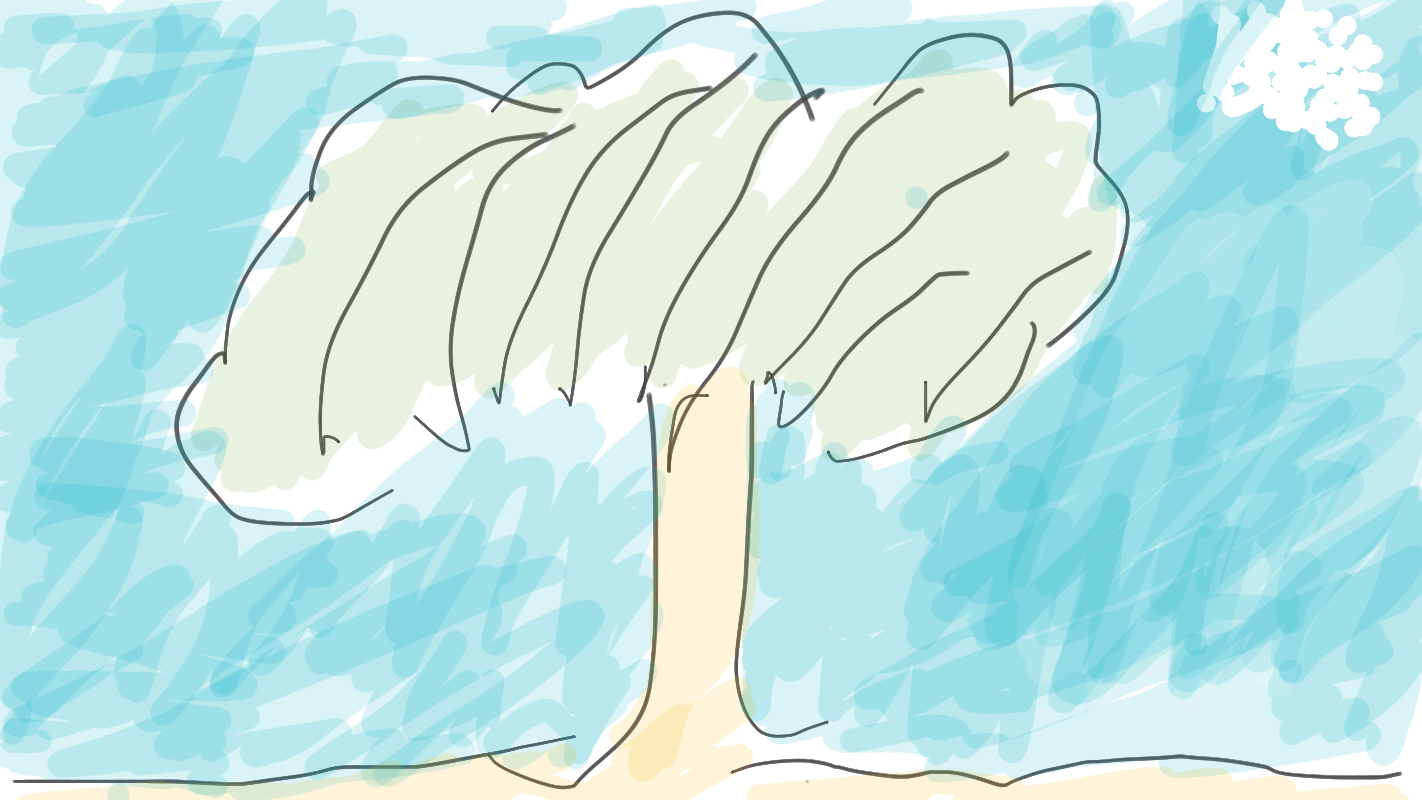
\includegraphics[width=1\textwidth]{tree.png}
            %
            \centering
            \\\ 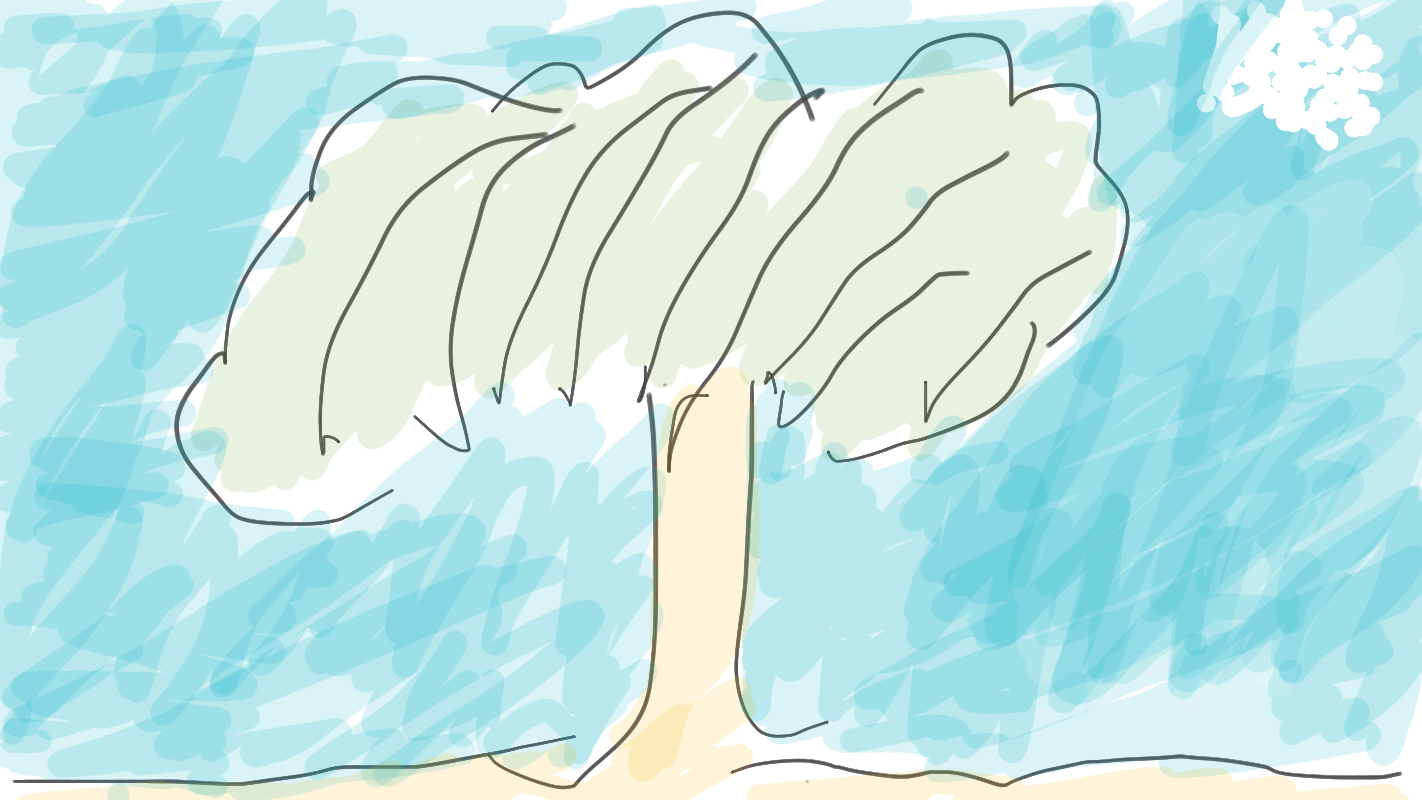
\includegraphics[width=0.75\textwidth]{tree.png}
            %Starting figure
            \begin{figure}[h]
            \centering
            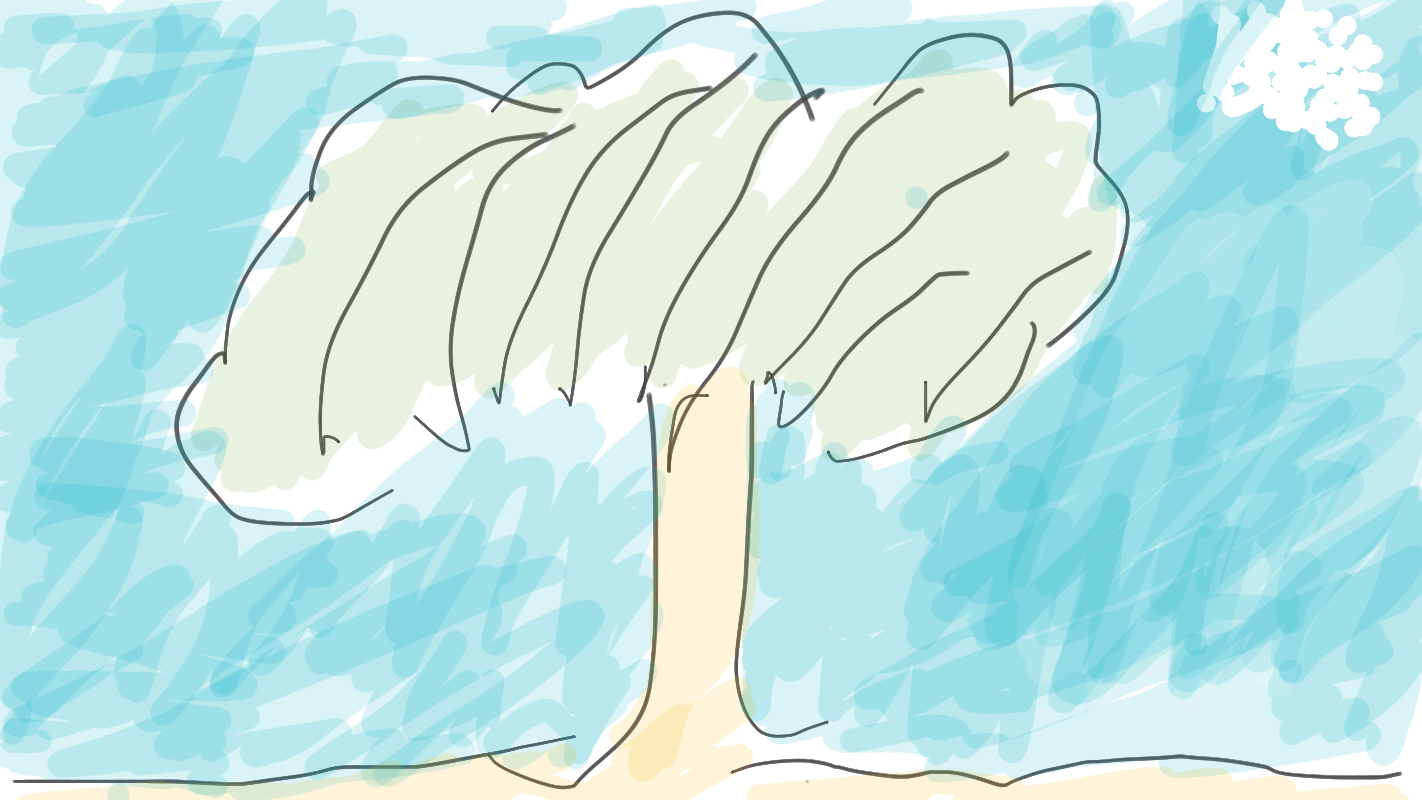
\includegraphics[width=0.8\textwidth]{tree.png}
            \caption{A nice plot.}
            \label{fig:tree1}
            As you can see in figure \ref{fig:tree1}, the function grows near the origin. This example is on page \pageref{fig:tree1}.
            \end{figure}
            %Ending figure
            \end{document}
            %Ending of this docement
